\documentclass[a4paper]{article} 

\input{head}

\usepackage{hyperref}

\begin{document}

\fancyhead[C]{}
\hrule \medskip
\begin{minipage}{0.295\textwidth} 
  \raggedright
  \scriptsize
  Michele Scomina \hfill\\   
  IN2000214\hfill\\
  mscomina@gmail.com\hfill\\
  michele.scomina@studenti.units.it
\end{minipage}
\begin{minipage}{0.4\textwidth} 
\centering 
\large 
\textbf{Docker - Cloud Storage}\\ 
\end{minipage}
\begin{minipage}{0.295\textwidth} 
\raggedleft
\today\hfill\\
\end{minipage}
\medskip\hrule 
\bigskip

\setlength{\parskip}{4pt}

\begin{abstract}
This is the report for Exercise 3. In this report we showcase a deployment procedure for a Cloud system,
as described in the \href{https://github.com/Foundations-of-HPC/Cloud-Basic-2023/blob/main/Assignments/Exercise.md}{GitHub repository}.
\end{abstract}

\section{Introduction}

This report describes the deployment of a cloud-based file storage
system based on Nextcloud. The system allows users to authenticate
and manage their own files, including uploading, downloading and
deleting files.

The system is deployed locally using Docker and Docker Compose, with
Nextcloud providing the file storage and web interface and MariaDB
providing the application database. Persistent Docker volumes are used
to ensure that application data and files survive container restarts.

\section{Architecture}

The deployment consists of two Docker containers. The first container
runs Nextcloud and provides the web interface and file-management
functionality. The second container runs MariaDB and stores Nextcloud's
application data.

The containers communicate through the Docker Compose network. The
MariaDB container is not exposed directly to the host, while the
Nextcloud container exposes its HTTP service through port 7489.

Two persistent Docker volumes are used. The \texttt{db\_data} volume
stores the MariaDB database, while \texttt{nextcloud\_data} stores the
Nextcloud installation and user files. Consequently, removing and
recreating the containers does not remove the persistent data.

Figure~\ref{fig:architecture} illustrates the main components of the
deployment and their relationships:

\begin{figure}[H]
    \centering
    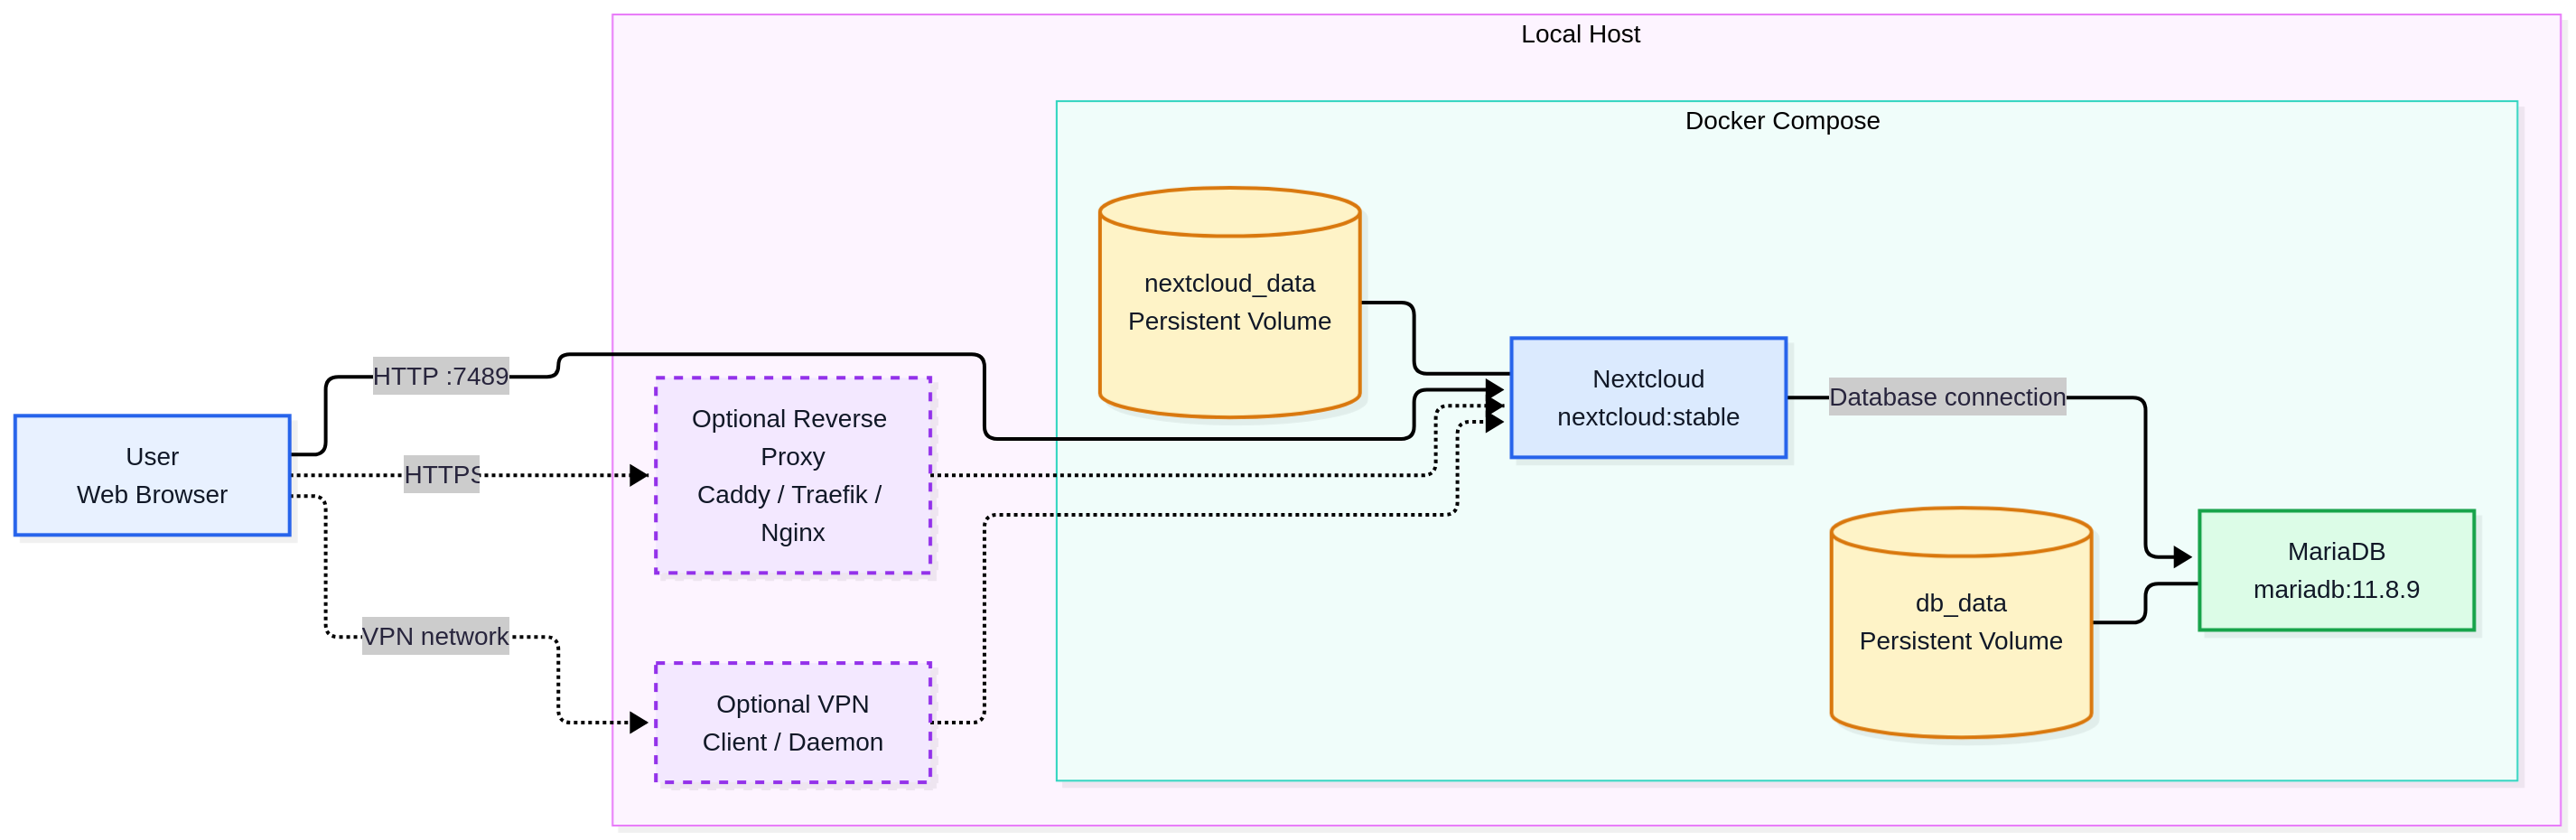
\includegraphics[width=0.98\textwidth]{mermaid_diagram.png}
    \caption{Architecture of the Nextcloud deployment.}
    \label{fig:architecture}
\end{figure}

\section{Deployment}

The system is deployed using Docker Compose. The complete deployment
configuration is provided in the repository in the
\texttt{docker-compose.yml} file.

The deployment uses the following images:

\begin{itemize}
\item \texttt{nextcloud:stable}, providing the cloud storage
application;
\item \texttt{mariadb:11.8.9}, providing the relational database.
\end{itemize}

The database is initialized using environment variables containing the
database name and credentials. Similarly, the initial Nextcloud
administrator account is configured through environment variables.

Sensitive values are not committed to the repository. Instead, the
repository contains a \texttt{.env.example} file which documents the
required configuration variables. The actual \texttt{.env} file is
excluded from version control.

The system can be deployed by first creating the environment
configuration and then starting the containers:

\begin{verbatim}
cp .env.example .env
docker compose up -d
\end{verbatim}

The running containers can be inspected with:

\begin{verbatim}
docker compose ps
\end{verbatim}

The Nextcloud web interface is available at
\texttt{http://localhost:7489}.

\section{User and File Management}

Nextcloud provides the authentication and authorization mechanisms
required by the exercise. Users can authenticate through the web
interface and each user has a separate file space.

The administrator account can create and manage users and therefore
provides the administrative functionality required by the assignment.
Regular users can upload, download and delete files belonging to their
own storage space.

No custom implementation of authentication or file management was
required, since these functionalities are provided by Nextcloud.

\section{Security}

\subsection{Authentication and Authorization}

Authentication and authorization are delegated to Nextcloud. Users
must authenticate before accessing their files, while administrative
operations are restricted to administrator accounts.

\subsection{Credential Management}

Database credentials and the initial administrator password are
provided through environment variables rather than being hard-coded
in the Docker Compose configuration. The actual \texttt{.env} file is
not committed to the repository. Its permissions could also be
restricted at the operating system level to prevent unauthorized
access. Ideally, database and administrator credentials should be
managed using a dedicated secrets mechanism, such as
\href{https://docs.docker.com/engine/swarm/secrets/}{Docker Secrets}.

As an additional security measure, the deployment could also be
implemented using Podman in rootless mode. This would allow the
containers to run without requiring root privileges on the host,
reducing the privileges available to container processes and limiting
the potential impact of a compromised container. Podman can be used
with common container workflows and could therefore be considered as
an alternative to Docker for deployments where minimizing
host-level privileges is a priority.

\subsection{Network Security and HTTPS}

The MariaDB service is only reachable from the Docker Compose network
and is not directly exposed through a host port. This reduces the
external attack surface of the deployment by preventing direct
connections to the database from outside the container network.

The local deployment currently uses HTTP because it is intended for
easy testing. For a production deployment, HTTPS should be provided
through a reverse proxy such as Caddy, Traefik, or Nginx. This would
ensure that communication between clients and the Nextcloud instance
is encrypted.

\subsection{Private Network Access}

Another possible deployment model is to use a private VPN such as
Tailscale
\href{https://tailscale.com/docs/features/tailscale-serve}{to expose
the service only to authorized devices}. In this scenario, the
Nextcloud instance would not need to be directly exposed to the public
Internet, reducing its external attack surface. Access to the service
could instead be restricted to devices connected to the private
network, while Nextcloud would continue to provide its own
application-level authentication and authorization.

This approach would be particularly suitable for a private deployment
where the storage service is intended to be accessed only by a
controlled set of users and devices. For a publicly accessible
production service, HTTPS and an appropriate reverse-proxy setup would
still be preferable.

\subsection{Additional Security Features}

Additional Nextcloud applications can be used to extend the security
and functionality of the platform. For example, the
\href{https://apps.nextcloud.com/apps/end_to_end_encryption}{End-to-End
Encryption application} can provide additional protection for
selected files.

\section{Performance Considerations}

The performance of the system depends primarily on the available CPU,
memory, storage and network bandwidth. File operations involving small
files are likely to be more affected by request and metadata overhead,
while large files are more dependent on storage and network throughput.

For a larger deployment, the performance could be evaluated by
generating concurrent upload and download requests and measuring
throughput, latency and resource utilization. The same approach could
be used to compare workloads involving small, medium and large files.

The current deployment is intended as a local demonstration and does
not attempt to reproduce a production-scale workload.

\section{Scalability}

The current deployment uses a single Nextcloud container and a single
MariaDB container, which is sufficient for a local deployment but would
not be suitable for a large number of users.

In a production environment, the system could be deployed using an
Infrastructure as a Service (IaaS) provider such as AWS, Microsoft
Azure or Google Cloud. Virtual machines or cloud container services
could be used to run multiple instances of the Nextcloud application,
with a load balancer distributing incoming requests between them. This
would allow the application layer to scale horizontally as the
workload grows.

The database could be moved to a managed or highly available database
service, while user files could be stored using scalable object
storage. Separating the application, database and file-storage layers
would allow each component to be scaled independently.

Caching could also be introduced to reduce repeated database and
application requests. Monitoring resource utilization and application
performance would allow resources to be increased or reduced according
to the actual workload.

\section{Cost Efficiency}

The proposed solution is based entirely on open-source software, such
as Nextcloud, MariaDB and Docker, resulting in no software licensing
costs.

The use of lightweight containers also helps keep resource usage low,
while monitoring can be configured to provide the necessary information
without introducing significant overhead. The local Docker deployment
is therefore particularly suitable for development and testing, as it
does not require any cloud infrastructure costs.

For a production deployment, cloud resources could be optimized
according to the workload. For example, auto-scaling groups could
dynamically adjust the number of application instances, while spot
instances could be used for workloads that can tolerate interruptions.
These approaches can reduce infrastructure costs while still allowing
the system to handle periods of increased demand.

\end{document}